% !TeX spellcheck = en_US
\chapter{Neuroscience}
\label{cha:neuroscience}

\section{Nervous System}
The nervous system has two main parts:
\begin{itemize}
	\item The \ac{CNS} is made up of the brain and spinal cord.
	\item The \ac{PNS} is made up of nerves that branch off from the spinal cord and extend to all parts of the body.
	\begin{itemize}
		\item Allows the \ac{CNS} to send and receive signal to other parts or our bodies
		\item Regulate involuntary functions, e.g., heartbeat, breathing, releasing hormones like adrenaline, opening the pupil in response to light, and regulating the digestive system.
	\end{itemize}
\end{itemize}

\subsection{Neuron}
The fundamental unit of the nervous system is nerve cell, \ac{aka} neuron.
\begin{figure}[hbt!]
	\centering
	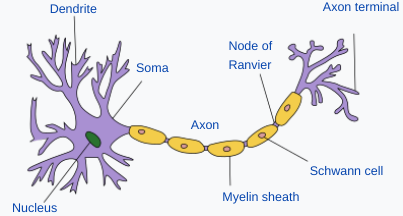
\includegraphics[width=0.72\textwidth]{neuron.png}
	\caption{Neuron structure}
\end{figure}
\begin{itemize}
	\item A \textit{neuron} has a cell body, which includes the cell nucleus, and extensions called \textit{axons} (/AK-sonz/) and \textit{dendrites} (/DEN-drahytz/).
	\item \textit{Synapse} (/SIN-aps/) is the space between the end of an axon and the tip of a dendrite from another neuron.
	\item Axons and dendrites allow neurons to communicate, even across long distances.
	\item Bundles of axons, called nerves, are found throughout the body.
	\item Neuron send a message to another neuron by
	\begin{itemize}
		\item Send an electrical signal down the length of its axon
		\item At the end of the axon, the electrical signal changes to a chemical signal, which is released with \textit{neurotransmitters} (/noor-oh-TRANS-mit-erz/) into the synapse
		\item The neighboring dendrite converts the chemical signal back into an electrical signal. 
	\end{itemize}
	\item \textit{Glia} (/GLEE-uh/), non-neuron cells, perform many important functions that keep the nervous system working properly
	\begin{itemize}
		\item Support and hold neurons in place
		\item Protect neurons
		\item Create myelin insulation called, which helps move nerve impulses
		\item Repair neurons and help restore neuron function
		\item Trim out dead neurons
		\item Regulate neurotransmitters
	\end{itemize}
\end{itemize}
\subsection{References}
\begin{itemize}
	\item \href{https://en.wikipedia.org/wiki/Nervous_system}{Wikipedia - Nervous System}
	\item \href{https://www.nichd.nih.gov/health/topics/neuro/conditioninfo/}{NIH - What are the parts of the nervous system?}
\end{itemize}

\section{The Brain}
\begin{itemize}
	\item \textit{Brain anatomy} is also called brain structure.\\
	Animals' brains have common structure:
	\begin{itemize}
		\item Forebrain
		\item Midbrain
		\item Hindbrain
		\item Spinal cord
	\end{itemize}
	\item \textit{Brain physiology} is also called as brain function.\\
	The closer we are to the spinal cord, the more basic the functions are, \eg, breathing, digest food.
\end{itemize}

\begin{figure}[hbt!]
	\centering
	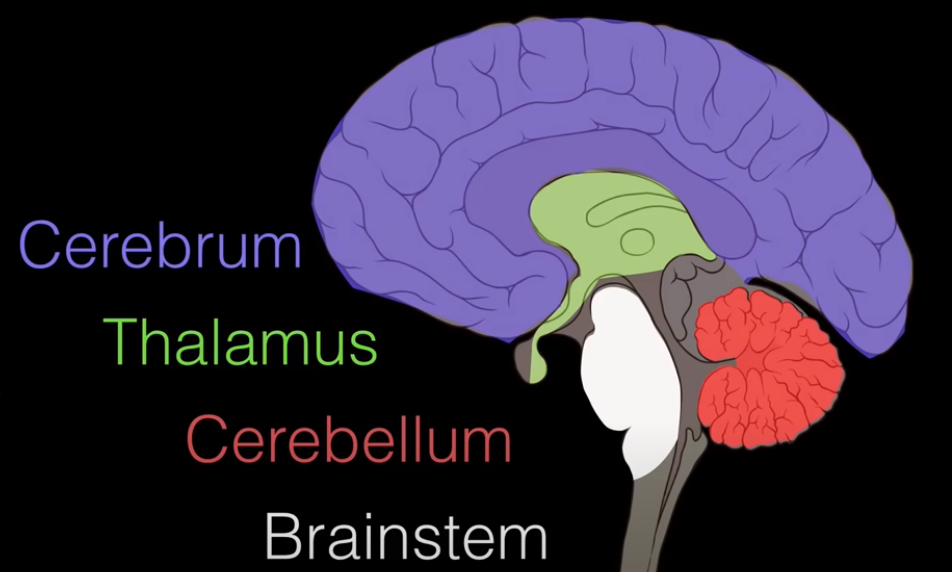
\includegraphics[width=0.52\textwidth]{brain-struct-1.png}
	\caption{Human's brain structure.}
\end{figure}

Human's brain structure:
\begin{itemize}
	\item \textit{Brainstem}
	\begin{itemize}
		\item Includes: \textit{midbrain, pons, medulla oblangata}
		\item Functions:
		\begin{itemize}
			\item Basic functions: breathing, circulation, digestion
			\item Sort in/out sensory information
		\end{itemize}
	\end{itemize}
	\item \textit{Cerebellum}: body control, motion memory
	\item \textit{Thalamus}: is like a router, sort data to the cerebrum
	\begin{itemize}
		\item Includes: \textit{hypothalamus}, \textit{posterior pituitary}
		\item Homeostasis for maintaining body temperature, circadian rhythm, \etc
	\end{itemize}
	\item \textit{Cerebrum}: 80\% of the brain
	\begin{itemize}
		\item Integrates different data
		\item Has two hemisphere, connected via \textit{corpus collosum}
		\item Divides into four lobes:
		\begin{itemize}
			\item Frontal lobe: personality, emotion, high-level thinking, controlling movements
			\item Parietal lobe (/puh.\textbf{rai}.uhtl/): sensation, deal and react with environment
			\item Occipital lobe (/uhk.\textbf{si}.puhtl/): vision, recognition of shapes, colors
			\item Temporal lobe: language, hearing, reading, memory, other senses
		\end{itemize}
		\item The parts on two side of the edge between frontal and parietal lobes are called:
		\begin{itemize}
			\item Somatosensory cortex: takes in sensation, makes sense of it
			\item Motor cortex: sends information out
		\end{itemize}
	\end{itemize}
\end{itemize}

\begin{figure}[hbt!]
	\centering
	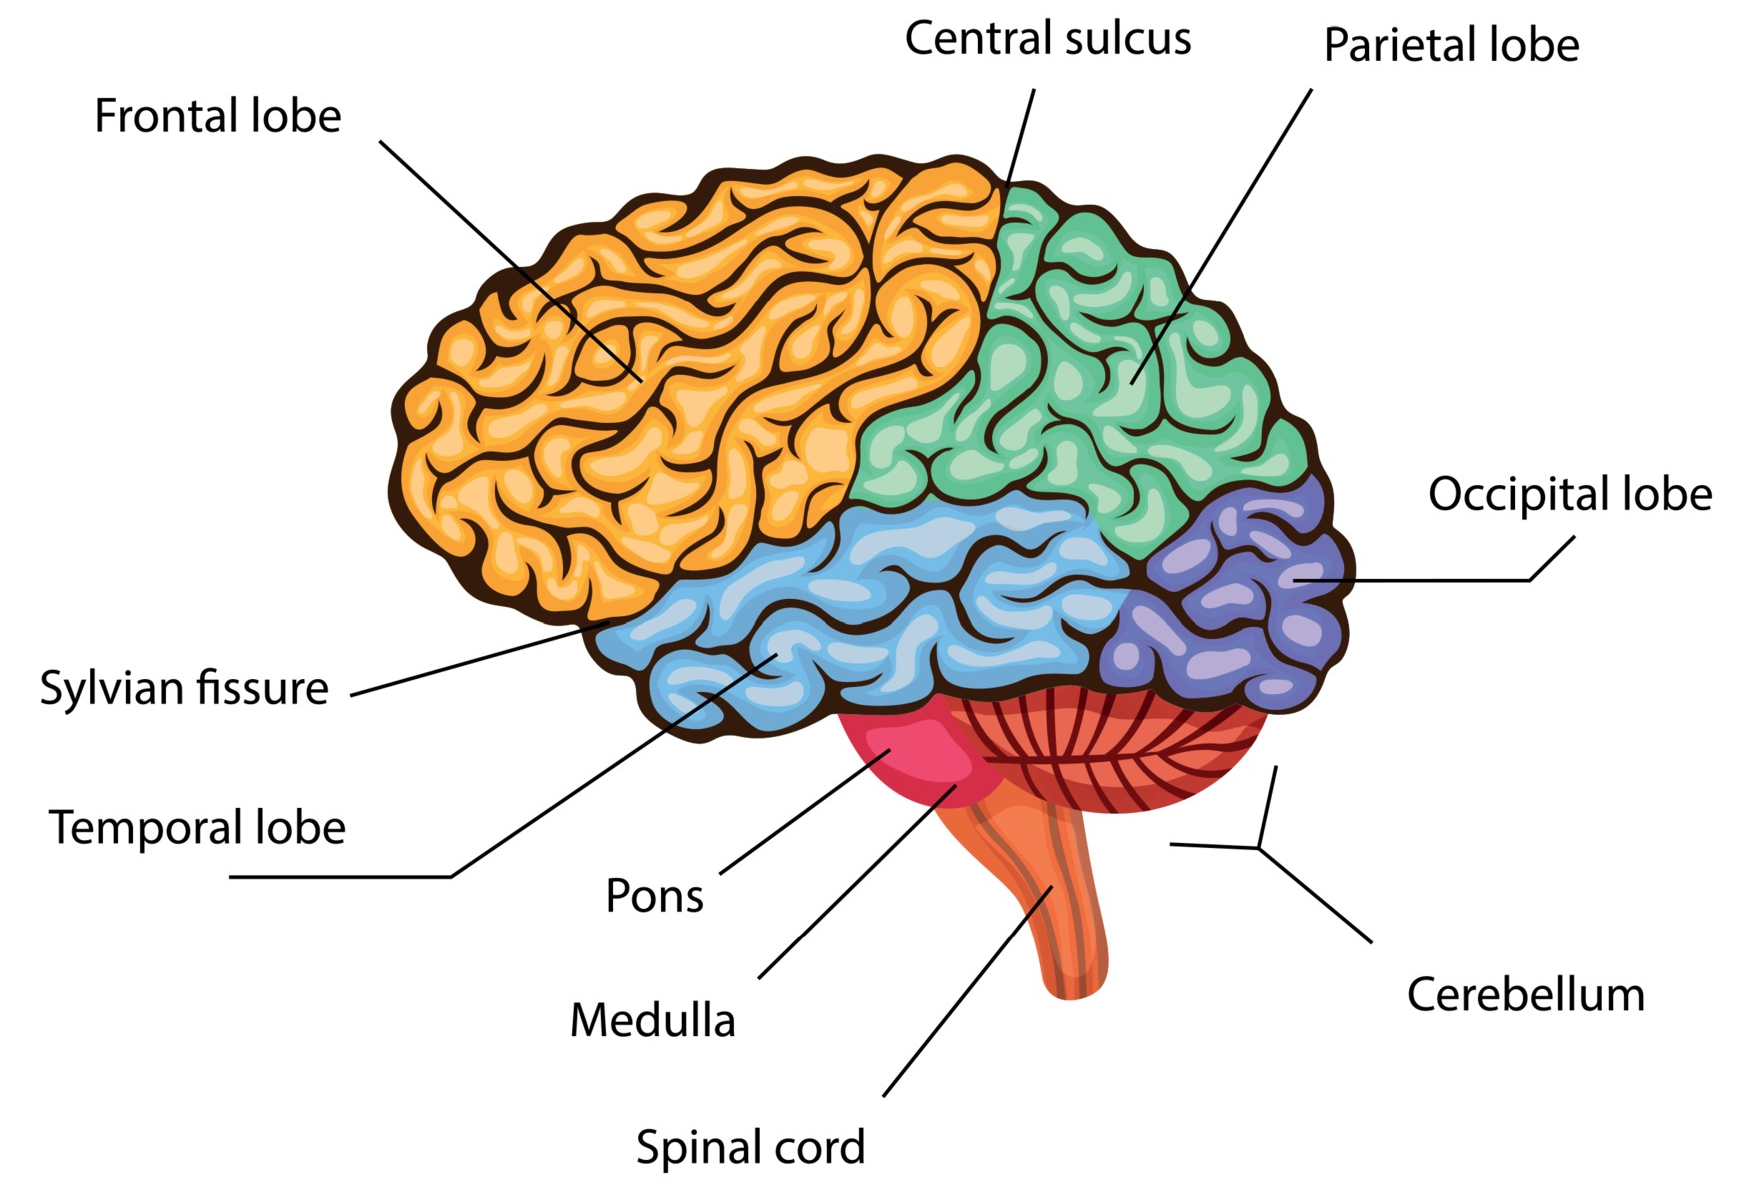
\includegraphics[width=0.72\textwidth]{brain-struct-2.png}
	\caption{Human's brain structure.}
	\label{fig:brain-struct-2}
\end{figure}

\subsection{References}
\begin{itemize}
	\item \href{https://en.wikipedia.org/wiki/Brain}{Wikipedia - Brain}
	\item \href{https://youtu.be/EeE7Fpg061I}{medXclusive Learning - Human Brain: Major Structures and their Functions}
	\item \href{https://youtu.be/kMKc8nfPATI}{Bozeman Science - The Brain}
\end{itemize}

\section{Brainwaves}
\begin{itemize}
	\item Clusters of neurons, which getting message/feedback from each other, start synchronize their firing patterns with others.
	\item This results in \textit{neural oscillations}, or \textit{brainwaves}, which are rhythmic or repetitive patterns of neural activity in the \ac{CNS}
\end{itemize}

\subsection{Categorization}
A non-inclusive list of types of oscillatory activity found in the central nervous system:
\begin{itemize}
	\item Delta waves (0.1-4Hz): technically links with deep sleep
	\item Theta waves (4Hz-7.5Hz): daydreaming, or meditation
	\item Mu waves (8Hz-12Hz): ??
	\item Alpha waves (7.5Hz-15Hz): awake, but relax
	\item Beta waves (12Hz-30Hz): awake, thinking about something
	\item Gamma waves (30Hz-100Hz): deeply focus
	\item At one, all waves are somewhat active, it's just that some waves are more dominant.
\end{itemize}
\begin{figure}[hbt!]
	\centering
	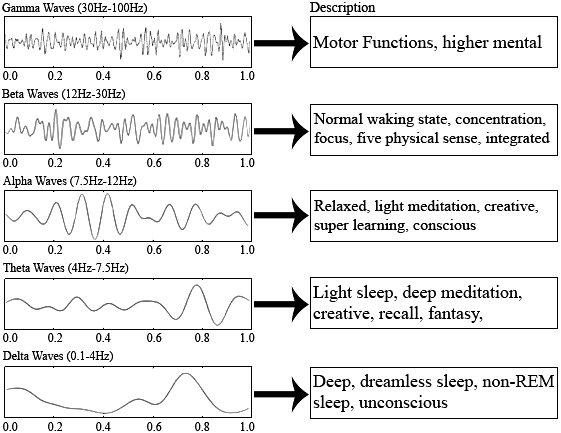
\includegraphics[width=0.72\textwidth]{brain-waves.png}
	\caption{Some of the common brainwaves.}
\end{figure}

\note
\begin{itemize}
	\item There are more than 5 types, check \href{https://en.wikipedia.org/wiki/Neural_oscillation}{Wikipedia - Neural oscillation}
	\item Each with different frequency and probably different functions in our brain.
	\item Generally, the higher the frequency, the more alert you are
\end{itemize}

\subsection{Comparison}
\todo{How to compare brain waves?}
\begin{itemize}
	\item \ac{FFT}
	\item Cross-correlation
\end{itemize}

\subsection{Brain Imaging Techniques}
\textit{Brain imaging techniques} are methods to measure these brainwaves. Some common methods with their pros and cons are (\figref{brain-imaging-techniques.png}):
\begin{itemize}
	\item \ac{EEG}:
	\[\begin{matrix*}[l]
		\color{Green} + \text{Inexpensive, portable, high temporal resolution}\\
		\color{red} - \text{Low spatial resolution}
	\end{matrix*}\]
	\item \ac{fMRI}
	\[\begin{matrix*}[l]
		\color{Green} + \text{Higher spatial resolution}\\
		\color{red} - \text{Low temporal resolution, high cost}
	\end{matrix*}\]
	\item \ac{ECoG}
	\[\begin{matrix*}[l]
		\color{Green} + \text{Higher spatial and temporal resolution}\\
		\color{red} - \text{Requires surgery, signals can degrade}
	\end{matrix*}\]
	\item \ac{LFP} and Spikes
	\[\begin{matrix*}[l]
		\color{Green} + \text{Very high spatial and temporal resolution}\\
		\color{red} - \text{Requires surgery, signals can degrade, high power consumption and latency}
	\end{matrix*}\]
\end{itemize}

\begin{figure}[hbt!]
	\centering
	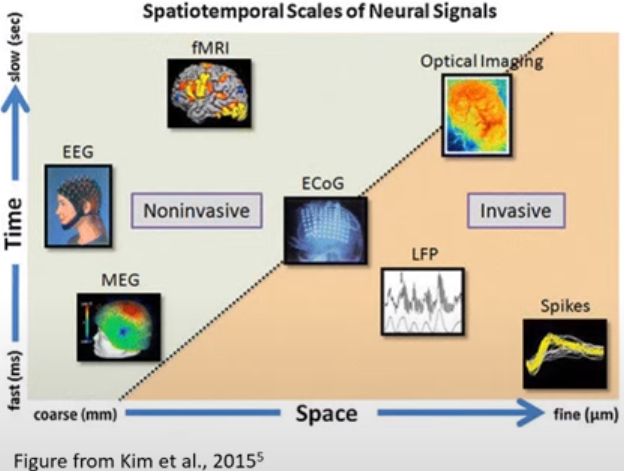
\includegraphics[width=0.72\textwidth]{brain-imaging-techniques.png}
	\caption{Different brain imaging techniques techniques vary in spatial and temporal resolution.}
	\label{brain-imaging-techniques.png}
\end{figure}

\subsection{References}
\begin{itemize}
	\item \href{https://youtu.be/LoGBCsFPNzU}{Microsoft Research | Developing a BCI based on Visual Imagery}
\end{itemize}

\section{Brain-Computer Interface}
\ac{BCI}, \ac{aka} \ac{BMI}, \ac{NMP}, are devices that transform neural signals into command signal to operate other physical systems.

\begin{figure}[hbt!]
	\centering
	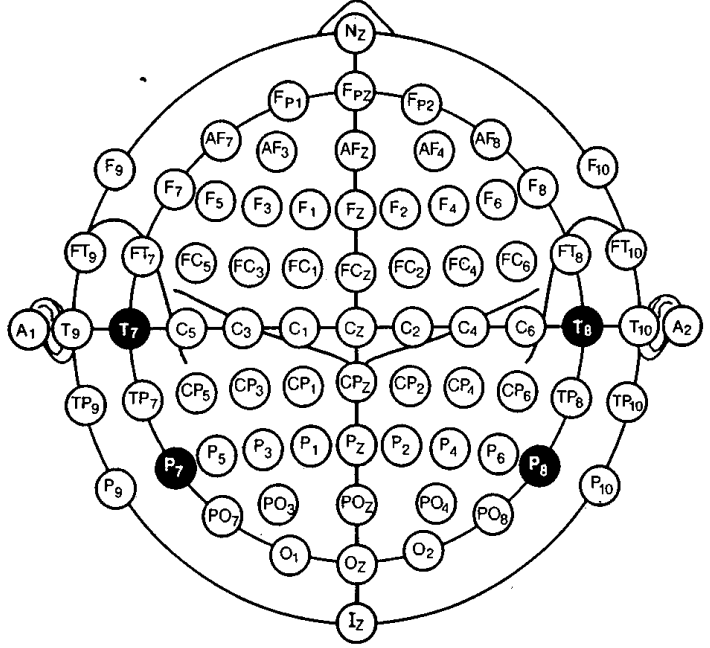
\includegraphics[width=0.72\textwidth]{bci-electrodes.png}
	\caption{The standard 64 scalp electrodes of \ac{BCI} system (view from above, subject's nose is at the top). Abbreviations: frontotemporal (FT), frontocentral (FC), temporal-posterior temporal (TP), centroparietal (CP), posterior temporo-occipital (PO), parieto-occipital (PO), anterior frontal (AF). \cite{sharbrough1991american}}
	\label{fig:bci-electrodes}
\end{figure}

\subsection{Paradigms}
There are two \ac{BCI} paradigms:
\begin{itemize}
	\item Evoked potentials: providing participants with external stimulus, then measure their responses.
	\begin{itemize}
		\item Visual P300
		\item Steady state visual evoked potential (SSVEP)
		\item Auditory stimuli: less studied
		\item Somatosensory (tactile) stimuli: less studied
	\end{itemize}
	\item Non-evoked potentials: participants engage in imagery and measure their brain activities.
	\begin{itemize}
		\item Motor imagery
		\begin{itemize}
			\item Sensorimotor rhythms (SMR): imagined movements of large body parts
			\item Imagined body kinematics (IBK): imagined movements of a single body part in a multi-dimensional space
		\end{itemize}
		\item Less studied non-evoked potentials
		\begin{itemize}
			\item Visual imagery: conceptual reconstruction of a perceptual experience
			\item Speed imagery: imagery of speed production
			\item Mental effort: mental object rotation, math calculations, \etc
		\end{itemize}
	\end{itemize}
\end{itemize}

\subsection{EEG Processing}
There are 3 types of feature extraction methods for EEG processing:

\begin{itemize}
	\item Spectral
	\begin{itemize}
		\item Frequency - domain analysis: Estimation of spectral power (stationary signals)
		\begin{itemize}
			\item \ac{PSD} (Welch's Periodogram)
			\item \ac{FFT}
		\end{itemize}		
		\item Time - frequency domain analysis\\
		Mother wavelets and wavelet transform
	\end{itemize}	
	\item Temporal
	\item Spatial
\end{itemize}

Microsoft Research:
\begin{enumerate}
	\item Collect raw EEG Data
	\item Channel selection (different electrodes in different brain areas)
	\item Apply filter, remove noise (power line noise)
	\item Artifact removal (eye, muscle movements)
	\item Epoch data
	\item Feature extraction
\end{enumerate}

\subsection{Motor Imagery}
\begin{itemize}
	\item \citeausm{wolpaw2000brain} used $\mu$ and $\beta$ waves from midpoint of the central sulcus (\figref{fig:brain-struct-2}) bilaterally to control computer cursor. It is probably using signal from C3 and C4 electrodes (\figref{fig:bci-electrodes})
	\item \citeausm{pfurtscheller2001motor}
	\item \citeausm{hoshino2021brain} used 14 EEG signals are measured at AF3, AF4, F3, F4, F7, F8, FC5, FC6, T7, T8, P7, P8, O1, and O2, which lie on all 4 lobes. Filter from 10Hz-50Hz ($\alpha. \beta, \gamma$ waves)
\end{itemize}

\subsection{Visual Imagery}
\subsection{Audio Imagery}
\subsection{References}
\begin{itemize}
	\item \href{https://en.wikipedia.org/wiki/Brain%E2%80%93computer_interface}{Wikipedia - Brain–computer interface}
	\item \href{https://youtu.be/LoGBCsFPNzU}{Microsoft Research | Developing a \ac{BCI} based on Visual Imagery}
	\item \citeaustitle{sharbrough1991american}
	\item \citeaustitle{wolpaw2000brain}
\end{itemize}

\section{TODO List}
\begin{itemize}
	\item How different is the brain waves when we concentrate on different things?
	\item How can we ensure, measure human concentration?
	\item How do the brain waves differ in varied context (quiet room, on the street, party, relax, focused)?
	\item How noise is the brain waves in the above context?
	\item How was the data collected? Can we augmented the brainwave dataset? If yes, how, augment irrelevant waves?
	\item EFP?	
\end{itemize}

\section{References}
\begin{itemize}
	\item \href{https://en.wikipedia.org/wiki/Nervous_system}{Wikipedia - Nervous System}
	\item \href{https://en.wikipedia.org/wiki/Neural_oscillation}{Wikipedia - Neural oscillation}
	\item \href{https://en.wikipedia.org/wiki/Brain%E2%80%93computer_interface}{Wikipedia - Brain–computer interface}
\end{itemize}